\section{Lifetime Repair \cite{AdventureOfALifetime}}
\label{app:lifetime_repair}

% \begin{algorithm}
%     \caption{FixLifetimes}
%     \textbf{Input}: a cargo manifest file CARGO\_MANIFEST for the whole project, extracted function EF \\
%     \textbf{Output}: patched extracted function EF'
%     \begin{algorithmic}[1]
%         \State $EF' \gets$ clone EF
%         \State $EF' \gets$ update EF' by annotating each borrow in EF'.params and EF'.ret with a fresh lifetime where none exists
%         \State $EF' \gets$ update EF' by adding the freshly introduced lifetimes to the list of lifetime parameters in EF'.sig
%         \Loop
%             \State $err \gets$ (cargo check CARGO\_MANIFEST).errors
%             \If{$err = \emptyset$}
%                 \State break
%             \EndIf
%             \State $suggestions \gets$ collect lifetime bounds suggestions from err
%             \If{$suggestions = \emptyset$}
%                 \State raise RefactorError
%             \EndIf
%             \State $EF' \gets$ apply suggestions to EF'
%         \EndLoop
%         \State collapse the cycles in the where clause of EF'.sig
%         \State apply elision rules
%     \end{algorithmic}
% \end{algorithm}

\begin{figure*}[h!]
    \centering
    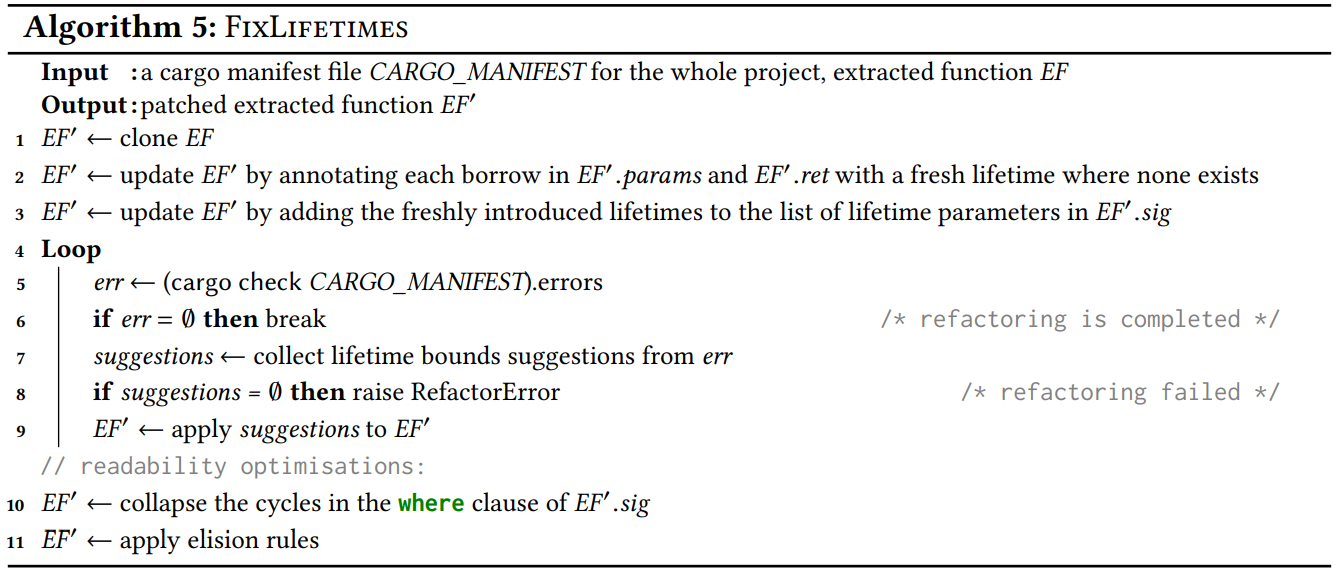
\includegraphics[width=\textwidth]{figures/algo_5.png}
    % \caption{Lifetime Repair}
    \label{fig:algo_5}
\end{figure*}